% !TEX root = ../Thesis.tex
\chapter{Introduction}

\textbf{Challenges in Program Analysis.} Symbolic execution is a powerful program analysis technique used for vulnerability discovery, test case generation, and software property verification.

Beyond security analysis, symbolic execution serves as a foundation for various software verification tasks, including bug detection, correctness checking, and automated program reasoning.

However, in large software systems, often lacking a well-defined analysis entry point, finding suitable starting points for symbolic execution is far from straightforward. Programs frequently serve a wide range of use cases, contain numerous execution paths, and can be expansive enough to obscure which code regions are security-critical and drive the core vulnerability landscape.

Moreover, symbolic execution faces a fundamental scalability challenge known as the ``path explosion problem''. As program complexity increases, the number of possible execution paths grows exponentially, quickly overwhelming computational resources and rendering the analysis intractable for real-world software systems. One recent example demonstrating this challenge is the analysis of complex libraries like OpenSSL, where millions of execution paths can emerge from relatively small input variations, making exhaustive analysis computationally prohibitive.

\begin{figure}[htbp]
    \centering
    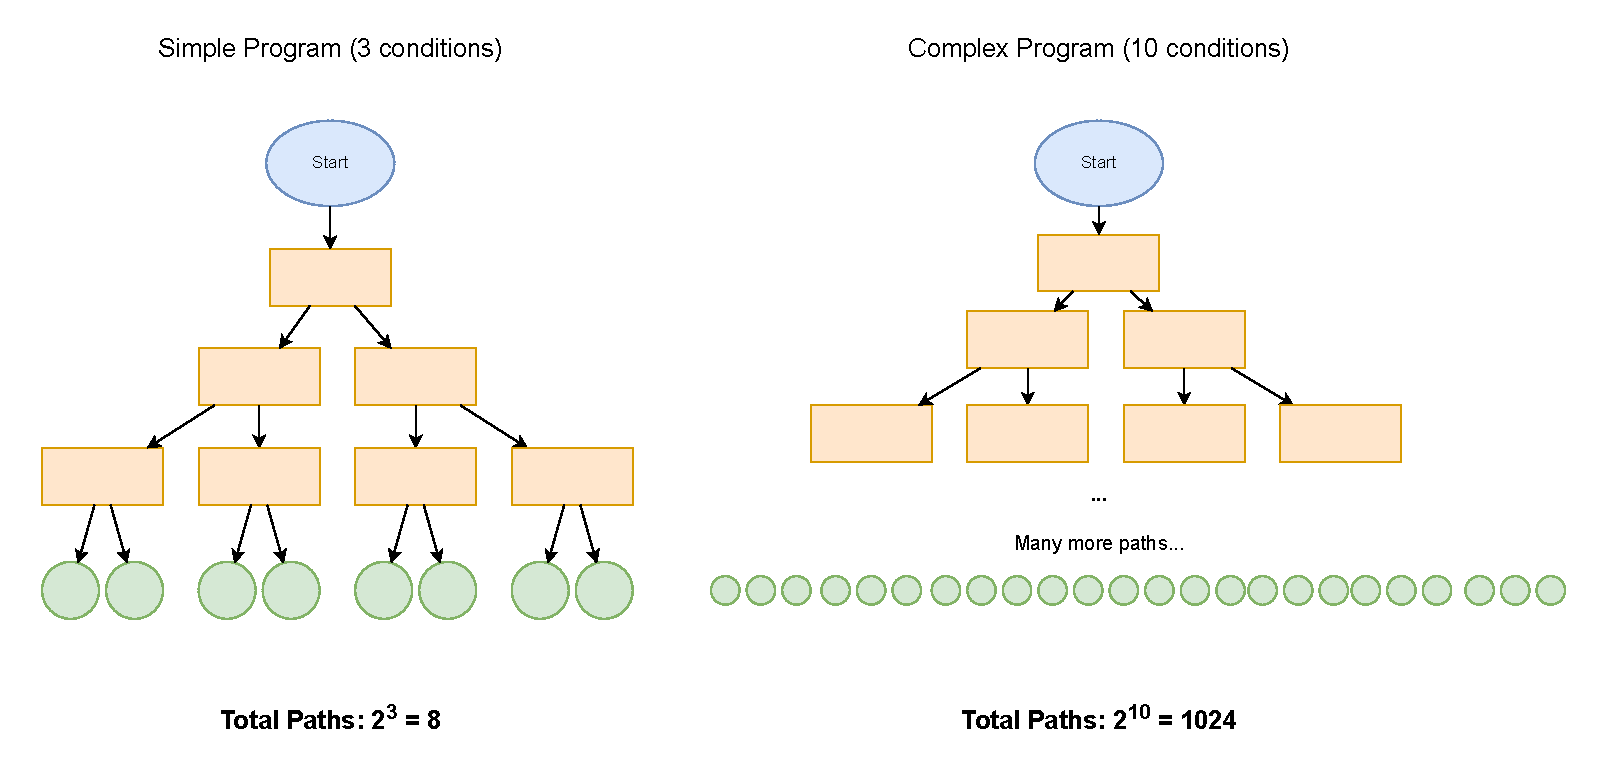
\includegraphics[width=\textwidth]{Figures/path_explosion_problem}
    \caption{Illustration of the path explosion problem: As program complexity increases from 3 to 10 conditions, the number of possible execution paths grows exponentially from 8 to 1024 paths.}
    \label{fig:path_explosion_problem}
\end{figure}

Despite the importance of efficient symbolic execution, practitioners lack an automated method to intelligently prioritize promising execution paths for security analysis. Manually determining where analysis should begin can be tedious and error-prone. The structure of even medium-sized programs can be extremely cluttered and overwhelming. Current symbolic execution engines typically employ uniform exploration strategies, treating all program paths with equal priority regardless of their potential security relevance, as Figure~\ref{fig:path_explosion_problem} illustrates with a simplified program control flow.

Addressing this issue could significantly enhance both the efficiency and thoroughness of symbolic execution for security testing.

% Suggestions
% Add after path explosion discussion:
\textbf{Taint Analysis Motivation:} Traditional symbolic execution treats all execution paths with equal priority, failing to distinguish between security-critical paths that process user input and auxiliary paths that handle internal program state. This uniform treatment leads to computational waste on paths unlikely to contain vulnerabilities.

\textbf{Thesis Overview.} This work presents TraceGuard\footnote{https://github.com/ruben-hutter/TraceGuard}, a novel approach that integrates taint analysis with symbolic execution to enable intelligent path prioritization. The methodology identifies and tracks data flow from critical sources such as user inputs and memory allocation sites, guiding the symbolic execution engine to focus computational resources on paths most likely to exhibit security-relevant behaviors. The main contributions of this thesis are:

\begin{itemize}
    \item \textbf{Taint-Guided Path Prioritization:} A novel integration of dynamic taint analysis with symbolic execution that uses taint propagation patterns to intelligently prioritize exploration of security-relevant execution paths.

    \item \textbf{Adaptive Scoring Algorithm:} A scoring mechanism that dynamically adjusts path priorities based on real-time taint analysis results, enabling the symbolic execution engine to focus computational resources on the most promising program regions.

    \item \textbf{Practical Implementation:} A complete implementation of the proposed approach using the angr symbolic execution framework, demonstrating the feasibility and effectiveness of taint-guided exploration in a production-quality tool.

    \item \textbf{Empirical Evaluation:} Comprehensive evaluation comparing the proposed approach against standard symbolic execution techniques, which will measure improvements in analysis efficiency, vulnerability discovery rate, and overall scalability.
\end{itemize}

% TODO: Check this when benchmarks are ready

The effectiveness of this optimization will be evaluated through extensive experimentation on representative programs, examining key metrics including runtime efficiency, path coverage quality, and vulnerability detection capabilities. Preliminary analysis indicates that the taint-guided approach can significantly reduce analysis time while maintaining or improving the detection of security-relevant program behaviors, making symbolic execution more practical for analyzing large and complex software systems.

The thesis is organized as follows:

\begin{itemize}
    \item \textbf{Chapter 2} reviews essential background concepts including symbolic execution, taint analysis, and the angr framework.
    \item \textbf{Chapter 3} presents the conceptual framework and theoretical algorithms underlying the taint-guided exploration strategy.
    \item \textbf{Chapter 4} details the practical implementation of the proposed approach, including integration with angr and the design of the scoring mechanism.
    \item \textbf{Chapter 5} presents a comprehensive evaluation of the approach, comparing its performance against standard symbolic execution techniques.
    \item \textbf{Chapter 6} discusses related work in symbolic execution optimization and path prioritization.
    \item \textbf{Chapter 7} concludes with a summary of contributions and implications for future research.
    \item \textbf{Chapter 8} explores potential extensions and future research directions.
\end{itemize}
